\documentclass{tufte-handout}

\title{CMPT 419/726 --- Machine Learning}

\author[Salehen Shovon Rahman]{Salehen Shovon Rahman}

%\date{28 March 2010} % without \date command, current date is supplied

%\geometry{showframe} % display margins for debugging page layout

\usepackage{graphicx} % allow embedded images
  \setkeys{Gin}{width=\linewidth,totalheight=\textheight,keepaspectratio}
  \graphicspath{{graphics/}} % set of paths to search for images
\usepackage{amsmath}  % extended mathematics
\usepackage{booktabs} % book-quality tables
\usepackage{units}    % non-stacked fractions and better unit spacing
\usepackage{multicol} % multiple column layout facilities
\usepackage{lipsum}   % filler text
\usepackage{fancyvrb} % extended verbatim environments
  \fvset{fontsize=\normalsize}% default font size for fancy-verbatim environments

% Standardize command font styles and environments
\newcommand{\doccmd}[1]{\texttt{\textbackslash#1}}% command name -- adds backslash automatically
\newcommand{\docopt}[1]{\ensuremath{\langle}\textrm{\textit{#1}}\ensuremath{\rangle}}% optional command argument
\newcommand{\docarg}[1]{\textrm{\textit{#1}}}% (required) command argument
\newcommand{\docenv}[1]{\textsf{#1}}% environment name
\newcommand{\docpkg}[1]{\texttt{#1}}% package name
\newcommand{\doccls}[1]{\texttt{#1}}% document class name
\newcommand{\docclsopt}[1]{\texttt{#1}}% document class option name
\newenvironment{docspec}{\begin{quote}\noindent}{\end{quote}}% command specification environment

\begin{document}

\maketitle% this prints the handout title, author, and date

\begin{abstract}
\noindent
Personal notes regarding machine learning.
\end{abstract}

%\printclassoptions

\section{Polynomial Curve Fitting}\label{sec:polynomial-curve-fitting}

\newthought{Here's an example machine learning problem}: try to find the best
polynomial that can potentially fit a set of data points, and have it be fit as
best as possible. This is known as the polynomial curve fitting problem, and
it's a supervised regression learning problem.

\begin{marginfigure}
  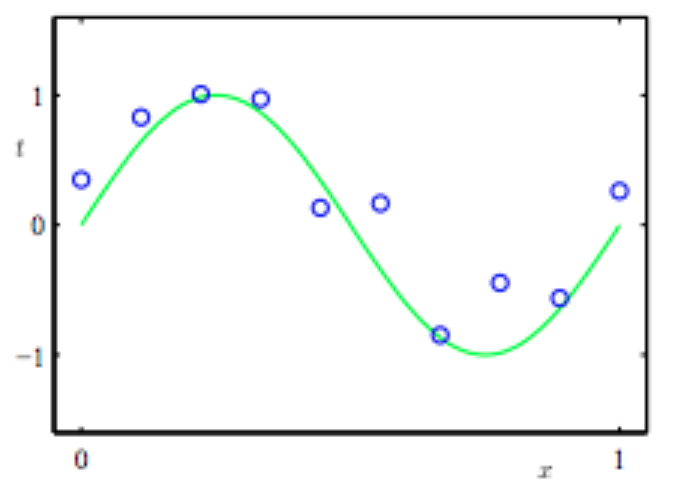
\includegraphics[width=\linewidth]{curvefitting.png}
  \caption{An example data set where we want to fit a polynomial curve into.}
\end{marginfigure}

\subsection{The Problem}\label{sec:headings}

\newthought{Suppose} we are given a training set of $N$ observations, $(x_{1},
x_{2}, \ldots, x_{N})$ and $(t_{1}, t_{2}, \ldots, x_{N})$, $x_{i}, t_{i} \in
\mathbb{R}$. We want to find a polynomial $y(x)$ that fits these data the best.

Let's start out by defining a $y(x, \mathbf{w})$.

\[
  y(x, \mathbf{w}) = w_0 + w_1x + w_2x^2 + \ldots + w_Mx^M =
  \sum\limits_{i = 1}^M(w_ix^i)
\]

How do we measure success? Or, a better question, for what values of the
coefficients $\mathbf{w}$ will yield the best results? To answer that, we define
an error function $E$.

\[
  E(\mathbf{w}) = \frac{1}{2}\sum\limits_{i = 1}^N(y(x_i, \mathbf{w}) - t_i)^2
\]

We then use the $\arg\min\limits_{x}f(x)$ function to find the value for the
parameter that yields the lowest value in a given function.

\[
  \mathbf{w}^* = \arg \min\limits_{\mathbf{w}}E(\mathbf{w})
\]

$\min\limits_{x} f(x)$ finds the lowest possible value for the
expression $f(x)$, while $\arg\min\limits_{x} f(x)$ finds the value for $x$
where $f(x)$ would be the lowest.

So, in other words, we want to find a $\mathbf{w}$ such that $E(\mathbf{w})$ is
the lowest among the set of all possible values of $\mathbf{w}$.

\newthought{Except}, the attempt at finding a value $\mathbf{w}^*$ such that
$E(\mathbf{w}^*) = 0$ can become problematic.

Earlier, we mentioned that we had an initial set of training data. However, for
most cases, when trying to fit the polynomial such that $E(\mathbf{w}^*) = 0$,
for the training set, we risk having it so that when a test data set is
introduced, the error function yields a high value. This is known as
\textit{overfitting}.

\begin{marginfigure}
  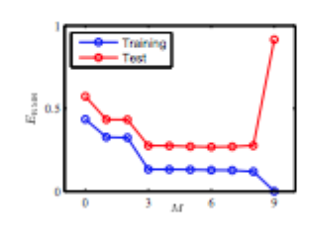
\includegraphics[width=\linewidth]{overfitting.png}
  \caption{As we can see, the first few polynomials of degree $N < 9$ fit the
    data fine, even when test data is introduced to the training set, but misses
    the mark entirely when $N = 9$. This is the result of overfitting.}
\end{marginfigure}

In the end of the day, although we want the curve to fit the data as best as
possible, we also want a \textit{genralization} derived from the given training.

\newthought{But first}, before we go ahead with finding a good gneralization,
for convenience, instead of just using the error function $E$, we use the
root-mean-square (RMS) error function, defined by

\[
  E_{\text{RMS}} = \sqrt{2E(\mathbf{w}^*)/N}
\]

According to the text book, \textit{Pattern Recognition and Machine Learning},
the reason why we are using RMS, is the following:

\begin{quote}
  [The] division by $N$ allows us to compare different sizes of data sets
  on an equal footing, and the square root ensures that $E_{\text{RMS}}$ is
  measured on the same scale (and in the same units) as the target variable $t$.
  (p. 7)
\end{quote}

Now, to actually tune our $\mathbf{w}$ for better generalization, we can split
our training data into two sets: training set and validation set. In the case of
finding the polynomial, the training set can be used to find each $w_i \in
\mathbf{w}$, and the validation set is used to optimize the complexity, which
can be represented by $M$ (the size of $\mathbf{w}$), or a $\lambda$, which
will be discussed later.

There are several techniques used to control overfitting.

\newthought{The first technique} to avoid overfitting is cross-validation.

Here, we group the data into separate sets. We first ``train'' our parameters to
a union of all the separated set, while leaving one out. Then we optimize by
including the one we initially excluded. Afterwards, we ``train'' again with a
new union of our sets, while leaving yet another one out, but including the one
that we initially left out, all the way until no sets are left to ``leave out''.

\newthought{And then}, there's regularization for controlling over-fitting.

Notice how the oscillation increases as $M$ increases? This is because the
magnitudes of the coefficients in $\mathbf{w}$ increases as $M$ increases.

\begin{marginfigure}
  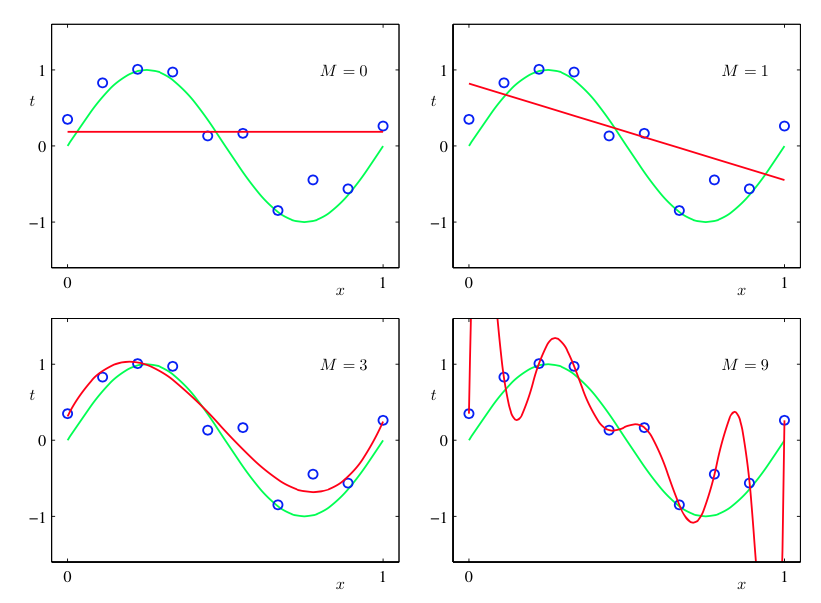
\includegraphics[width=\linewidth]{oscillations.png}
  \caption{Visually, we see that the oscillation increases as $M$ increases.}
\end{marginfigure}

\begin{table}[h]
  \footnotesize%
  \begin{center}
    \begin{tabular}{lrrrr}
      \toprule
       & $M = 0$ & $M = 1$ & $M = 6$ & $M = 9$ \\
      \midrule
      $w_0$ & 0.19 &  0.82 &   0.31 &        0.35 \\
      $w_1$ &      & -1.27 &   7.99 &      232.37 \\
      $w_2$ &      &       & -25.43 &    -5321.83 \\
      $w_3$ &      &       &  17.37 &    48568.31 \\
      $w_4$ &      &       &        &  -231639.30 \\
      $w_5$ &      &       &        &   640042.26 \\
      $w_6$ &      &       &        & -1061800.52 \\
      $w_7$ &      &       &        &  1042400.18 \\
      $w_8$ &      &       &        &  -557682.99 \\
      $w_9$ &      &       &        &   125201.43 \\
      \bottomrule
    \end{tabular}
  \end{center}
  \caption{For higher values of $M$, we see the magnitude of $w_i$ increasing}
  \label{tab:font-sizes}
\end{table}

In order to avoid high coefficient magnitudes, we can ``penalize'' them using
a modified error function, by adding a $\frac{\lambda}{2}\|\mathbf{w}\|$ term
to the original error function.

\[
  \widetilde{E}(\mathbf{w}) =
    \frac{1}{2}\sum\limits_{i = 1}^N(y(x_i, \mathbf{w}) - t_i)^2
      + \frac{\lambda}{2}\|\mathbf{w}\|
    = E(\mathbf{w}) + \frac{\lambda}{2}\|\mathbf{w}\|
\]

If we are to now apply the error function to our trials, we see that the
ceofficient are no longer large.

\begin{table}[h]
  \footnotesize%
  \begin{center}
    \begin{tabular}{lrrr}
      \toprule
       & $\ln\lambda = -\infty$ & $\ln\lambda = -18$ & $\ln\lambda = 9$ \\
      \midrule
      $w_0$ &        0.35 &   0.35 &  0.13 \\
      $w_1$ &      232.37 &   4.74 & -0.05 \\
      $w_2$ &    -5321.83 &  -0.77 & -0.06 \\
      $w_3$ &    48568.31 & -31.93 & -0.05 \\
      $w_4$ &  -231639.30 &  -3.89 & -0.03 \\
      $w_5$ &   640042.26 &  55.28 & -0.02 \\
      $w_6$ & -1061800.52 &  41.32 & -0.01 \\
      $w_7$ &  1042400.18 & -45.95 & -0.00 \\
      $w_8$ &  -557682.99 & -91.53 &  0.00 \\
      $w_9$ &   125201.43 &  72.68 &  0.01 \\
      \bottomrule
    \end{tabular}
  \end{center}
  \caption{For higher values of $\lambda$, the coefficient magnitudes are much
    lower, possibly even near $0$}
  \label{tab:font-sizes}
\end{table}

\begin{fullwidth}
  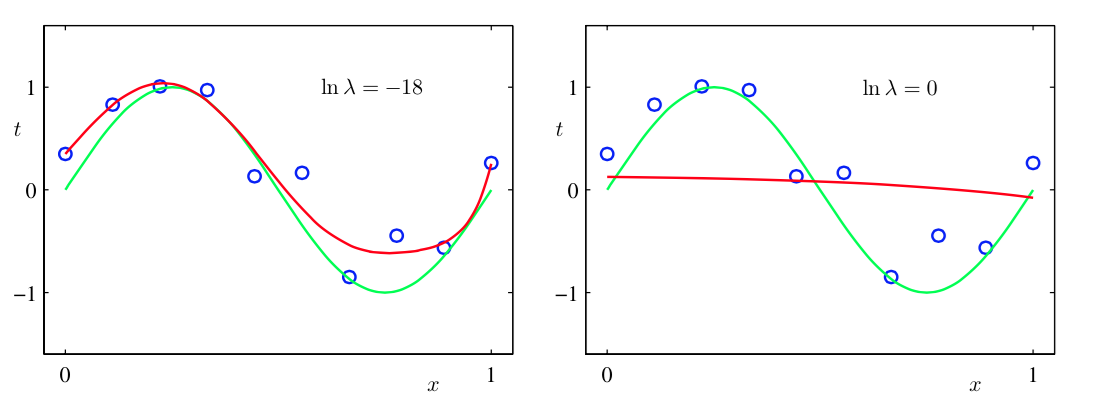
\includegraphics[width=\linewidth]{lambda.png}
  \small{\itshape{As you can see here, even for $M = 9$, previously, the
  polynomial curve deviated wildly, which could have potentially yielded high
  error values relative to new potential data}}
\end{fullwidth}

\begin{figure*}[h]
  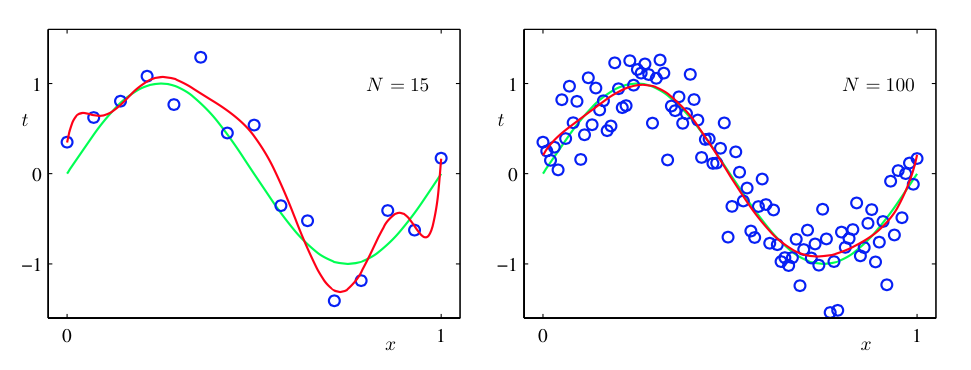
\includegraphics[width=\linewidth]{moredata.png}%
  \caption{On the left, we see an \emph{attempt} at having the curve fitted to
  the data we have so far; on the right, we see more data added, and the curve
  appears show a much better approximation.}
\end{figure*}

\newthought{Finally}, there's the third option: just get more data! A rule of
thumb is that the number of datapoints should not be any less than five times
the number of adaptive parameters.

\section{Probability Theory}

\subsection{Random Variables}

\newthought{The term} ``random variable'' is can be misleading. A random
variable is not a variable at all. Instead, it's a mapping from a
\emph{random event} to a possible outcome.

So here's an example random variable:

\[
  X =
    \begin{cases}
      1 \text{ if } \text{heads} \\
      0 \text{ if } \text{tails} \\
    \end{cases}
\]

As we can see here, $X$ is a mapping from the set $\{ \text{heads},
\text{tails} \}$, to the set $\{ 1, 0 \}$.

More informally, a random variable is a ``label'' to a given element of a set of
possible events.

To add to the confusion, when we say that we have an event from our random
variable (for example, an event from $X$ defined above), we express it as
$X = 0$ or $X = 1$, etc.

The end purpose of random variables is to derive a probability distribution
given a value $x \in \{ \text{Range of X} \}$. So, going back to the above
head/tail example, if we wanted to express the probability of getting heads, we
write $p(X = 1)$, likewise, for expressing the probability of getting tails, we
write $p(X = 0)$, and so and so forth.

The purpose of using random variables is for us to easily be able to write
inequalities inside our probability expression. So, for instance, let's define a
random variable $Y$ that contains a mapping of a list of combinations of two
dices to the sum of their faces. We can easily express the probability of a
roll, for example, a value greater than 10, like so: $p(Y > 10)$.

\section{Figures and Tables}\label{sec:figures-and-tables}

Figure~\ref{fig:fullfig} is an example of the \Verb|figure*|
environment and figure~\ref{fig:textfig} is an example of the normal
\Verb|figure| environment.

\begin{figure*}[h]
  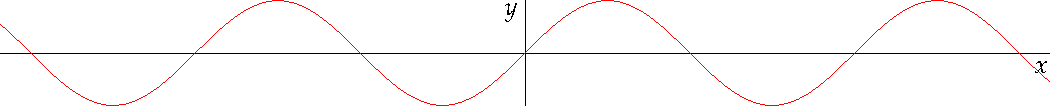
\includegraphics[width=\linewidth]{sine.pdf}%
  \caption{This graph shows $y = \sin x$ from about $x = [-10, 10]$.
  \emph{Notice that this figure takes up the full page width.}}%
  \label{fig:fullfig}%
\end{figure*}

\begin{figure}
  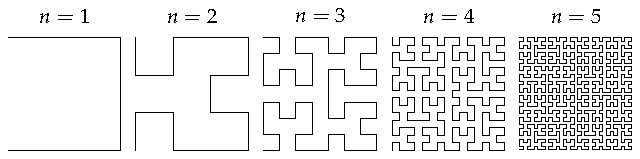
\includegraphics{hilbertcurves.pdf}
%  \checkparity This is an \pageparity\ page.%
  \caption{Hilbert curves of various degrees $n$.
  \emph{Notice that this figure only takes up the main textblock width.}}
  \label{fig:textfig}
  %\zsavepos{pos:textfig}
  \setfloatalignment{b}
\end{figure}

Table~\ref{tab:normaltab} shows table created with the \docpkg{booktabs}
package.  Notice the lack of vertical rules---they serve only to clutter
the table's data.

\begin{table}[ht]
  \centering
  \fontfamily{ppl}\selectfont
  \begin{tabular}{ll}
    \toprule
    Margin & Length \\
    \midrule
    Paper width & \unit[8\nicefrac{1}{2}]{inches} \\
    Paper height & \unit[11]{inches} \\
    Textblock width & \unit[6\nicefrac{1}{2}]{inches} \\
    Textblock/sidenote gutter & \unit[\nicefrac{3}{8}]{inches} \\
    Sidenote width & \unit[2]{inches} \\
    \bottomrule
  \end{tabular}
  \caption{Here are the dimensions of the various margins used in the Tufte-handout class.}
  \label{tab:normaltab}
  %\zsavepos{pos:normaltab}
\end{table}

\section{Full-width text blocks}

In addition to the new float types, there is a \docenv{fullwidth}
environment that stretches across the main text block and the sidenotes
area.

\begin{Verbatim}
\begin{fullwidth}
Lorem ipsum dolor sit amet...
\end{fullwidth}
\end{Verbatim}

\begin{fullwidth}
\small\itshape\lipsum[1]
\end{fullwidth}

\section{Typography}\label{sec:typography}

\subsection{Typefaces}\label{sec:typefaces}
If the Palatino, \textsf{Helvetica}, and \texttt{Bera Mono} typefaces are installed, this style
will use them automatically.  Otherwise, we'll fall back on the Computer Modern
typefaces.

\subsection{Letterspacing}\label{sec:letterspacing}
This document class includes two new commands and some improvements on
existing commands for letterspacing.

When setting strings of \allcaps{ALL CAPS} or \smallcaps{small caps}, the
letter\-spacing---that is, the spacing between the letters---should be
increased slightly.\cite{Bringhurst2005}  The \Verb|\allcaps| command has proper letterspacing for
strings of \allcaps{FULL CAPITAL LETTERS}, and the \Verb|\smallcaps| command
has letterspacing for \smallcaps{small capital letters}.  These commands
will also automatically convert the case of the text to upper- or
lowercase, respectively.

The \Verb|\textsc| command has also been redefined to include
letterspacing.  The case of the \Verb|\textsc| argument is left as is,
however.  This allows one to use both uppercase and lowercase letters:
\textsc{The Initial Letters Of The Words In This Sentence Are Capitalized.}



\section{Installation}\label{sec:installation}
To install the Tufte-\LaTeX\ classes, simply drop the
following files into the same directory as your \texttt{.tex}
file:
\begin{quote}
  \ttfamily
  tufte-book.cls\\
  tufte-common.def\\
  tufte-handout.cls\\
  tufte.bst
\end{quote}

% TODO add instructions for installing it globally



\section{More Documentation}\label{sec:more-doc}
For more documentation on the Tufte-\LaTeX{} document classes (including commands not
mentioned in this handout), please see the sample book.

\section{Support}\label{sec:support}

The website for the Tufte-\LaTeX\ packages is located at
\url{https://github.com/Tufte-LaTeX/tufte-latex}.  On our website, you'll find
links to our \smallcaps{svn} repository, mailing lists, bug tracker, and documentation.

\bibliography{sample-handout}
\bibliographystyle{plainnat}



\end{document}
